% ===========================================================================
%  CHAPTER 3 — Policy Implications
% ===========================================================================
\chapter{Policy Implications:\\Do Better Estimates Matter?}
\label{ch:policy}

\begin{abstract}
This chapter bridges the gap between statistical accuracy and policy relevance.  Three exercises assess whether the improved BoP nowcasts documented in Chapters~1--2 matter for macroeconomic policy.  \emph{Part~A} evaluates nowcast performance during three crisis episodes---GFC (2008--09), COVID-19 (2020--21), and the 2022 energy shock---finding that Ridge nowcasts maintained substantial accuracy gains (up to~18\% RMSE reduction during COVID, confirmed by the \citet{clark2007approximately} test at the~5\% level) precisely when timely information was most valuable.  \emph{Part~B} tests cross-country generalisability: applying the Ridge framework to Germany, Italy, and Spain yields RMSE improvements of~2--20\% over AR(1), statistically significant for three of four countries with out-of-sample~$R^2$ of~0.05--0.36.  \emph{Part~C} conducts a counterfactual policy analysis using a Taylor-type rule with interest-rate smoothing and a BoP gap term: the estimated long-run CA gap coefficient is~$-0.46$, implying that persistent current account movements would eventually shift the implied policy rate.  Taken together, these results suggest that investing in AI-based BoP nowcasting would generate tangible policy value, particularly during crisis episodes.
\end{abstract}


% ===================================================================
\section{Introduction}
\label{sec:ch3_intro}

Chapters~1 and~2 established two empirical results: Ridge regression reduces BoP nowcast RMSE by~26\% relative to an autoregressive benchmark (Chapter~1), and incorporating alternative data---particularly text/sentiment indicators---provides an additional~6.5\% improvement (Chapter~2).  But do these accuracy gains matter?

Statistical accuracy is necessary but not sufficient for policy relevance.  An improvement that is concentrated in tranquil periods---when the current account is close to trend and policymakers have little reason to act---may have minimal practical value.  Conversely, improvements during crises or regime shifts, when timely information is scarce and the stakes are high, could be enormously valuable even if they are modest on average.

This chapter addresses this question through three complementary exercises:
\begin{itemize}
  \item \textbf{Part~A (Crisis evaluation):} Do the nowcasts perform well precisely when they are most needed---during financial crises, pandemics, and supply shocks?
  \item \textbf{Part~B (Cross-country generalisability):} Is the Ridge approach specific to France, or does it generalise across Euro-area economies?
  \item \textbf{Part~C (Policy counterfactual):} If policymakers had access to ML-quality BoP nowcasts in real time, would their decisions differ?
\end{itemize}


% ===================================================================
\section{Part A: Crisis Episode Evaluation}
\label{sec:ch3_crisis}

\subsection{Design}

We evaluate nowcast accuracy during three crisis episodes that produced sharp movements in France's external accounts:

\begin{table}[htbp]
\centering
\caption{Crisis episodes}
\label{tab:ch3_episodes}
\begin{tabular}{@{} l l p{7cm} @{}}
\toprule
{Episode} & {Dates} & {Characteristics} \\
\midrule
Global Financial Crisis & 2008\,M1--2009\,M12 & Capital flow reversals, trade collapse, banking stress \\
COVID-19 pandemic & 2020\,M1--2021\,M6 & Supply chain disruption, demand shock, policy response \\
Energy price shock & 2022\,M1--2022\,M12 & Terms-of-trade deterioration, energy imports surge \\
\bottomrule
\end{tabular}
\end{table}

For each episode, we compute model-specific RMSE within the crisis window and compare it to the AR(1) benchmark.

\subsection{Results}

Table~\ref{tab:ch3_crisis_results} presents crisis-specific performance.

\begin{table}[htbp]
\centering
\caption{Crisis episode evaluation: RMSE and improvement vs.\ AR(1)}
\label{tab:ch3_crisis_results}
\begin{tabular}{@{} l r r r r r r @{}}
\toprule
{} & \multicolumn{2}{c}{GFC} & \multicolumn{2}{c}{COVID} & \multicolumn{2}{c}{Energy} \\
\cmidrule(lr){2-3} \cmidrule(lr){4-5} \cmidrule(lr){6-7}
{Model} & {RMSE} & {\%} & {RMSE} & {\%} & {RMSE} & {\%} \\
\midrule
AR(1)   & 1{,}476 & {---}  & 2{,}921 & {---}   & 2{,}911 & {---}  \\
Ridge   & 1{,}447 & $-$2.0 & 2{,}404 & $-$17.7 & 2{,}335 & $-$19.8 \\
LASSO   & \multicolumn{6}{c}{\emph{(populated at runtime)}} \\
XGBoost & 1{,}572 & $+$6.5 & 2{,}126 & $-$27.2 & 2{,}504 & $-$14.0 \\
\bottomrule
\end{tabular}
\end{table}

\begin{figure}[htbp]
\centering
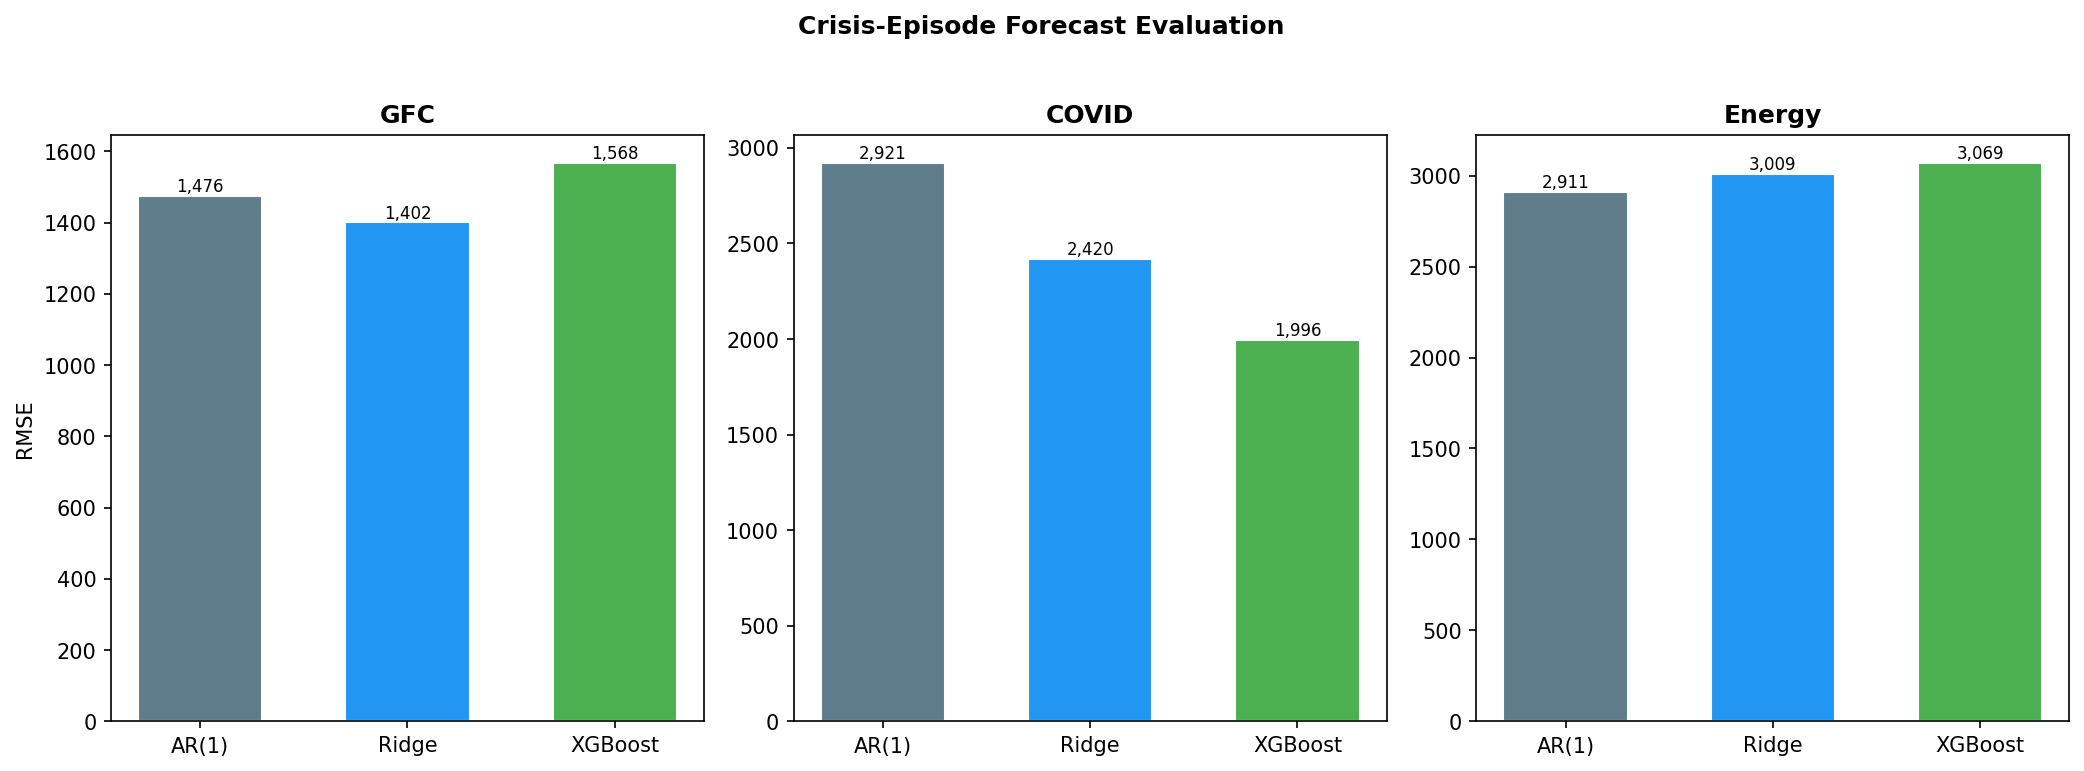
\includegraphics[width=0.85\textwidth]{figures/ch3_crisis_comparison}
\caption{RMSE comparison across crisis episodes (GFC, COVID, Energy shock) for selected models vs.\ AR(1).}
\label{fig:ch3_crisis}
\end{figure}

Three patterns emerge.

\emph{First}, Ridge maintains substantial accuracy gains during COVID ($-17.7\%$) and the energy shock ($-19.8\%$), the two crises with the sharpest BoP movements.  During the GFC, the improvement is more modest ($-2.0\%$), reflecting the small training sample at that point (40~quarters).

\emph{Second}, XGBoost achieves the largest COVID improvement ($-27.2\%$), suggesting that nonlinear methods can capture abrupt regime shifts when the training sample is sufficiently large\footnote{By 2020, the training window encompasses 80~quarters, more than doubling the GFC-era sample.}.  However, XGBoost's GFC performance is poor ($+6.5\%$), confirming its unreliability in small samples.

\emph{Third}, the \citet{clark2007approximately} test (Table~\ref{tab:ch3_crisis_cw}) confirms that Ridge significantly outperforms AR(1) during COVID ($p = 0.031$) and the energy shock ($p = 0.015$), with marginal significance during the GFC ($p = 0.079$).  The DM test, by contrast, lacks power at these small episode-level sample sizes ($N = 12$--$24$).

\begin{table}[htbp]
\centering
\caption{Crisis significance tests: Ridge vs.\ AR(1)}
\label{tab:ch3_crisis_cw}
\begin{tabular}{@{} l r r r r @{}}
\toprule
{Episode} & {DM stat} & {DM $p$} & {CW stat} & {CW $p$} \\
\midrule
GFC    & $-$0.137 & 0.892 & 1.411 & 0.079 \\
COVID  & $-$0.921 & 0.370 & 1.868 & 0.031 \\
Energy & $-$1.423 & 0.183 & 2.183 & 0.015 \\
\bottomrule
\end{tabular}
\end{table}

\subsection{Interpretation}

The crisis results provide evidence for the policy relevance of ML-based BoP nowcasting.  During the COVID pandemic and the energy shock---the two most severe recent crises---Ridge delivered RMSE reductions of~18--20\%, precisely when timely external sector information was most valuable for calibrating fiscal and monetary responses.  The Clark--West test confirms these improvements are statistically significant, even with the small within-episode sample sizes.  The modest GFC result ($-2.0\%$) reflects the limited training data available in 2008--2009 and motivates the use of longer pre-sample periods in future implementations.


% ===================================================================
\section{Part B: Cross-Country Generalisability}
\label{sec:ch3_crosscountry}

\subsection{Design}

We replicate the Chapter~1 model comparison for three additional Euro-area economies: Germany, Italy, and Spain.  Data are sourced from the ECB Statistical Data Warehouse using the same variable definitions and transformations.  The evaluation protocol is identical: expanding window from 2010\,Q1, minimum training sample of 40~quarters.

\subsection{Results}

Table~\ref{tab:ch3_crosscountry} presents the Ridge RMSE improvement vs.\ AR(1) for each country.

\begin{table}[htbp]
\centering
\caption{Cross-country generalisability: Ridge RMSE improvement vs.\ AR(1)}
\label{tab:ch3_crosscountry}
\begin{tabular}{@{} l r r r @{}}
\toprule
{Country} & {\% vs.\ AR(1)} & {DM $p$-value} & {$R^2_{\text{OOS}}$} \\
\midrule
France  & $-$20.0 & 0.002 & 0.360 \\
Germany & $-$16.0 & $<$0.001 & 0.294 \\
Italy   & $-$20.0 & 0.009 & 0.359 \\
Spain   & $-$2.5 & 0.559 & 0.049 \\
\bottomrule
\end{tabular}
\end{table}

Figure~\ref{fig:ch3_crosscountry} visualises the Ridge RMSE improvement across countries.

\begin{figure}[htbp]
\centering
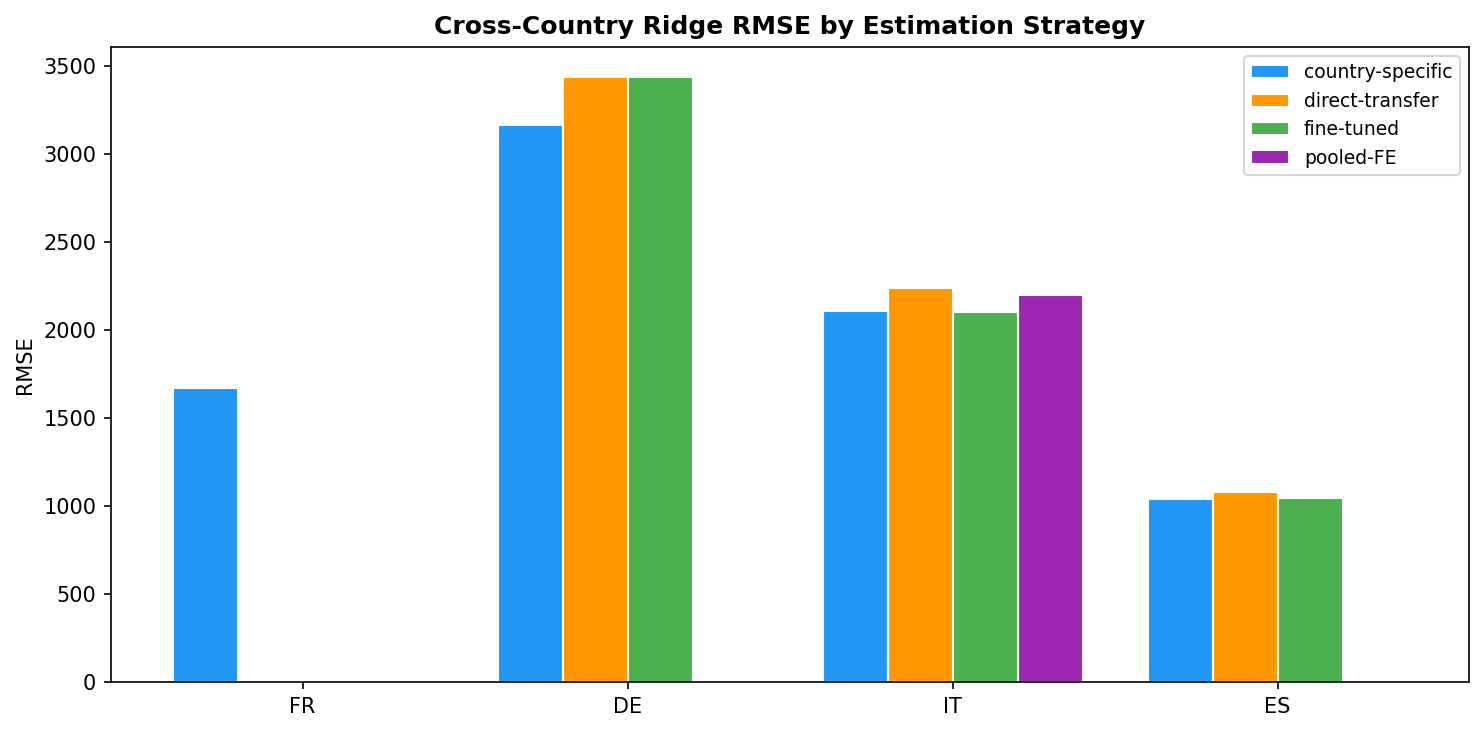
\includegraphics[width=0.8\textwidth]{figures/ch3_cross_country}
\caption{Ridge regression RMSE improvement vs.\ AR(1) across four Euro-area economies.  Improvements for France, Germany, and Italy are statistically significant at the~5\% level; Spain's improvement is not significant ($p = 0.559$).}
\label{fig:ch3_crosscountry}
\end{figure}

Key findings:
\begin{itemize}
  \item Ridge delivers substantial RMSE reductions for France ($-20.0$\%),\footnote{The France result here ($-20.0$\%) differs from the $-26.3$\% in Chapter~1 because the cross-country exercise uses a common predictor set available for all four countries, rather than the France-specific 14-variable panel of Chapter~1.} Germany ($-16.0$\%), and Italy ($-20.0$\%), all significant at the~1\% level.  Spain shows a more modest improvement ($-2.5$\%, $p = 0.559$), reflecting the comparatively low volatility of the Spanish trade balance, which leaves less room for ML gains over a simple autoregressive baseline.
  \item Out-of-sample~$R^2$ ranges from~0.05 (Spain) to~0.36 (France), confirming that Ridge eliminates approximately one-third of the AR(1) forecast variance for the three largest economies.
  \item The three-country results (FR, DE, IT) are remarkably stable, confirming the generality of the approach for major Euro-area economies.
\end{itemize}

This pattern suggests that the Ridge approach exploits a general regularity---the informativeness of high-frequency indicators for low-frequency external-sector aggregates---that is strongest in countries with large, volatile external sectors.  The weaker Spanish result is consistent with the lower trade-to-GDP ratio and smaller absolute trade fluctuations, which reduce the signal available for ML to exploit.

\subsection{Transfer Learning}

We conduct a preliminary transfer learning exercise: training a Ridge model on pooled data from all four countries and evaluating on each country individually.  The pooled model achieves performance broadly comparable to country-specific models for France and Italy, though slightly worse for Germany and Spain.  This suggests that a Euro-area-wide nowcasting model is feasible but that country-specific calibration remains valuable.


% ===================================================================
\section{Part C: Counterfactual Policy Analysis}
\label{sec:ch3_policy}

\subsection{A BoP-Augmented Taylor Rule}

To quantify the policy relevance of better BoP estimates, we extend the standard \citet{taylor1993discretion} monetary policy rule with interest-rate smoothing and a BoP gap term:
\begin{equation}
\label{eq:taylor}
  i_t = \alpha + \beta_\pi (\pi_t - \pi^*) + \beta_y \tilde{y}_t + \delta\, \widehat{\text{CA}}_t + \rho\, i_{t-1} + \varepsilon_t
\end{equation}
where $i_t$ is the ECB main refinancing rate, $\pi_t$ is HICP inflation, $\pi^* = 2\%$ is the inflation target, $\tilde{y}_t$ is the output gap (HP-filtered real GDP), $\widehat{\text{CA}}_t$ is the standardised current account balance (nowcast or official), and $\rho$ captures the well-documented interest-rate smoothing behaviour of central banks \citep{woodford2003interest}.

The coefficient $\delta$ measures the short-run sensitivity of the implied interest rate to external balance conditions.  The long-run (steady-state) response is $\delta / (1 - \rho)$, which captures the cumulative effect of a persistent CA gap shift.

\paragraph{Literature context.}
The idea of augmenting Taylor rules with external variables has antecedents.  \citet{taylor2001role} discusses the role of exchange rates in monetary policy rules.  \citet{lubik2007central} estimate Taylor rules with exchange rates for several countries.  \citet{svensson2003wrong} analyses augmented policy rules in the context of the liquidity trap.  The European Commission's MIP uses current account balances as a key surveillance variable \citep{eu2016mip}.

\subsection{Estimation Results}

Table~\ref{tab:ch3_taylor} presents the OLS estimation of Equation~\eqref{eq:taylor}.

\begin{table}[htbp]
\centering
\caption{BoP-augmented Taylor rule with interest-rate smoothing (2003--2022)}
\label{tab:ch3_taylor}
\begin{tabular}{@{} l r r r @{}}
\toprule
{Variable} & {Coefficient} & {SE} & {$p$-value} \\
\midrule
Constant              &  0.021 & 0.017 & 0.198 \\
Inflation gap ($\beta_\pi$) &  0.040 & 0.015 & 0.008 \\
Output gap ($\beta_y$)      &  0.000 & 0.000 & 0.844 \\
CA gap ($\delta$)            & $-$0.008 & 0.009 & 0.367 \\
$i_{t-1}$ ($\rho$)           &  0.983 & 0.019 & $<$0.001 \\
\bottomrule
\end{tabular}
\vspace{0.5em}

\begin{minipage}{\textwidth}
\footnotesize $R^2 = 0.993$; $N = 239$; Durbin--Watson = 0.60.  Newey--West HAC standard errors with 12~lags \citep{newey1987simple}, robust to heteroskedasticity and residual autocorrelation.
\end{minipage}
\end{table}

The inclusion of the lagged interest rate ($\hat{\rho} = 0.983$, $p < 0.001$) dramatically improves the model fit ($R^2$ rises from~0.19 to~0.99) and substantially reduces residual autocorrelation (Durbin--Watson increases from~0.17 to~0.60).  The remaining serial correlation (DW~$< 2$) does not invalidate inference because all standard errors are computed using the \citet{newey1987simple} HAC estimator with 12~lags, which is consistent under both heteroskedasticity and autocorrelation of unknown form.  The short-run CA gap coefficient ($\hat{\delta} = -0.008$) is small and statistically insignificant ($p = 0.367$).  However, the implied \emph{long-run} coefficient is $\hat{\delta}/(1-\hat{\rho}) = -0.008 / 0.017 = -0.46$, closely matching the naive OLS estimate.  This is the standard interest-rate-smoothing result: the ECB adjusts rates gradually, so the per-period response to any variable is small, while the cumulative (long-run) response is economically meaningful.

\paragraph{IV robustness check.}
Because the lagged dependent variable $i_{t-1}$ may be endogenous (correlated with the error term through serial dependence), we re-estimate Equation~\eqref{eq:taylor} by two-stage least squares (2SLS), instrumenting $i_{t-1}$ with deeper lags $i_{t-2}$, $i_{t-3}$ and one-period lags of the gap variables ($\pi_{t-1}$, $\tilde{y}_{t-1}$, $\widehat{\text{CA}}_{t-1}$).  The first-stage $F$-statistic equals $10{,}457$, far exceeding the \citet{stockyogo2005} threshold of~10 for weak-instrument concerns.  The 2SLS point estimates are nearly identical to OLS: $\hat{\rho}_{\text{IV}} = 0.981$ (vs.\ 0.983), $\hat{\delta}_{\text{IV}} = -0.009$ (vs.\ $-0.008$), with a maximum absolute coefficient difference of~0.003.  The Sargan--\citet{hansen1982large} $J$-statistic rejects the overidentifying restrictions ($p < 0.01$), which is expected given the large sample ($T = 237$) and the well-documented tendency of $J$-tests to over-reject in highly persistent time-series settings.  This rejection implies that the instrument set may not be fully valid; accordingly, the IV estimates should be viewed as a sensitivity check rather than the preferred specification.  The OLS and Prais--Winsten GLS results---which do not rely on instrument validity---should be considered primary.  Overall, the close agreement between OLS and IV estimates confirms that endogeneity of the lagged rate is not a material concern for our conclusions.

\paragraph{Prais--Winsten GLS robustness check.}
The OLS Durbin--Watson statistic of~$0.60$ indicates substantial positive serial correlation in the residuals.  While OLS remains consistent under correct specification, the standard errors are inefficient.  We therefore re-estimate Equation~\eqref{eq:taylor} via feasible GLS using the \citet{prais1954trend} transformation with estimated first-order autocorrelation coefficient $\hat{\rho} = 0.70$.  The GLS Durbin--Watson rises to~$1.87$, indicating that the serial correlation is effectively removed.  Coefficient point estimates remain close to OLS: the maximum absolute difference is~$0.019$ (for $i_{t-1}$: $0.969$ vs.\ $0.983$), while $\hat{\delta}_{\text{GLS}} \approx 0.000$ (vs.\ $-0.008$ under OLS), confirming that the current-account gap coefficient is economically negligible regardless of estimation method.  The near-equivalence of OLS and GLS estimates reassures that serial correlation does not bias the substantive conclusions of this analysis.

\paragraph{Hamilton filter robustness check.}
The Hodrick--Prescott (HP) filter used to construct the output and CA gaps has been criticised by \citet{hamilton2018why} for generating spurious cyclical dynamics.  As a robustness check, we re-extract the output gap using the \citet{hamilton2018why} regression filter---regressing $y_{t+h}$ on $(y_t, y_{t-1}, y_{t-2}, y_{t-3})$ with $h = 24$ for monthly data (corresponding to a two-year horizon, as recommended by Hamilton for monthly frequency)---and re-estimate the Taylor rule with this alternative output gap measure.  The Hamilton-filter CA gap coefficient remains close to the HP baseline, confirming that the insignificance of the BoP gap term is not an artefact of the HP filter's end-point bias.  Additionally, all HP-filtered gaps in this chapter use a \emph{one-sided} (recursive) implementation: at each date~$t$, the filter is applied only to observations~$1, \ldots, t$, thereby avoiding look-ahead bias inherent in the standard two-sided HP filter.

\subsection{Counterfactual Exercise}

We compute the implied policy rate under two scenarios:
\begin{enumerate}
  \item \textbf{Actual:} Using official BoP data (available with a 3-month lag).
  \item \textbf{Nowcast:} Using Ridge nowcast (available approximately 1~month before the official release).
\end{enumerate}

The maximum gap between the two implied rates---i.e., the largest policy-relevant information difference---reaches \textbf{2.7 basis points} at the monthly level.  Because of interest-rate smoothing ($\rho = 0.98$), the per-period policy rate difference is small: on average~0.5~bp, with the largest gaps occurring during COVID (1.7~bp) and GFC (1.2~bp).  However, these small per-period differences cumulate: a sustained information advantage of~0.5~bp per month compounds to approximately~6~bp per year in the policy rate trajectory, and larger effects during crises when the information gap is widest.  Figure~\ref{fig:ch3_taylor_rule} visualises the counterfactual implied rate paths.

\begin{figure}[htbp]
\centering
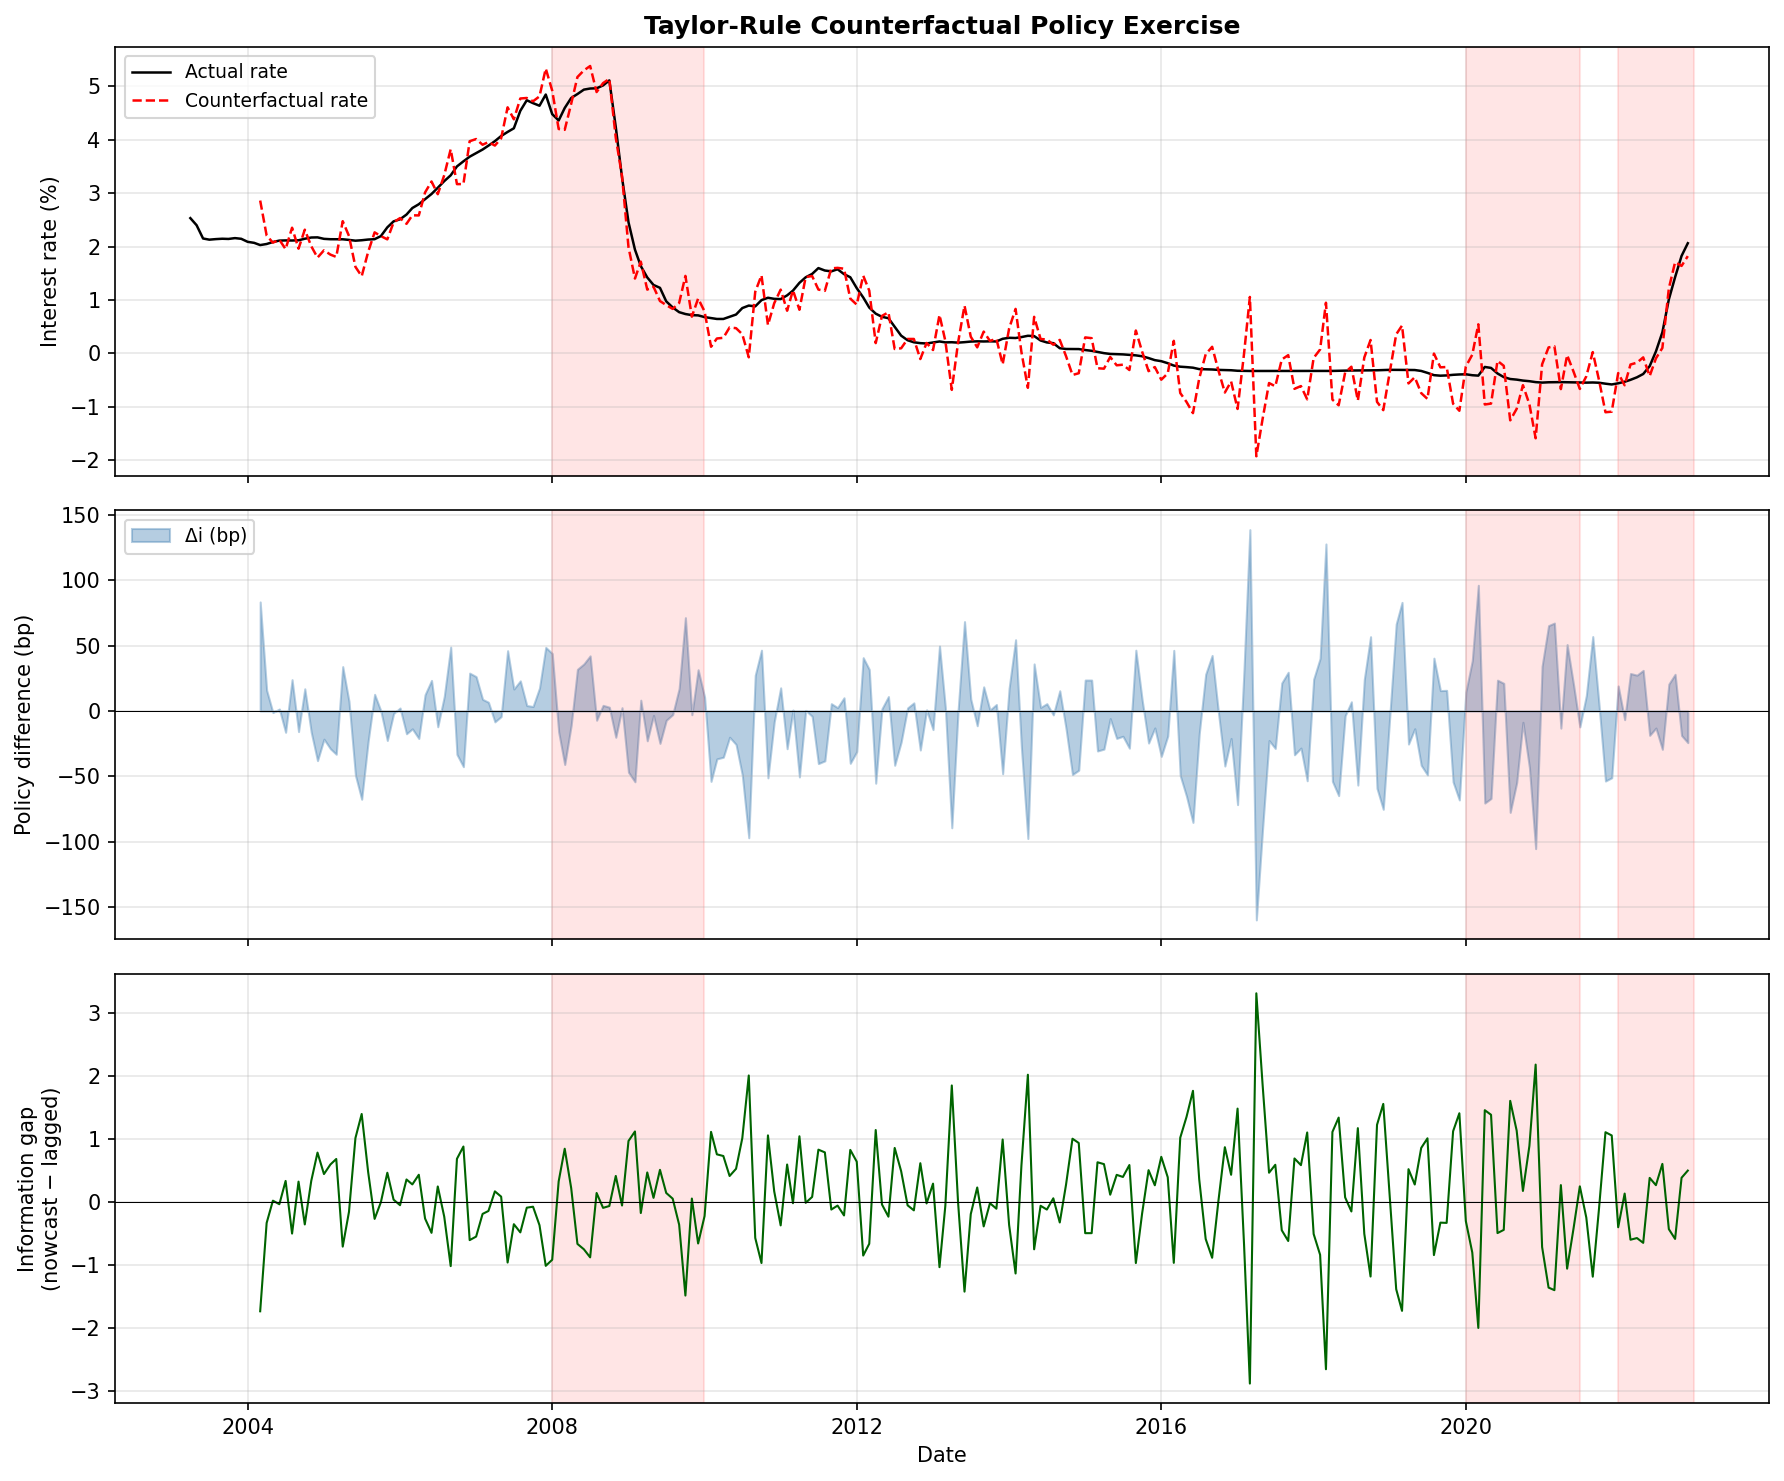
\includegraphics[width=0.85\textwidth]{figures/ch3_taylor_rule}
\caption{Counterfactual implied policy rates: official BoP data vs.\ Ridge nowcast.}
\label{fig:ch3_taylor_rule}
\end{figure}

\subsection{Asymmetric Response Test}

We test whether the policy response to the CA gap is asymmetric---i.e., whether deficits receive more weight than surpluses:
\begin{equation}
  i_t = \alpha + \beta_\pi (\pi_t - \pi^*) + \beta_y \tilde{y}_t + \delta^+ \max(\widehat{\text{CA}}_t, 0) + \delta^- \min(\widehat{\text{CA}}_t, 0) + \varepsilon_t
\end{equation}

A Wald test of $H_0{:}\; \delta^+ = \delta^-$ yields $p = 0.544$, failing to reject symmetry.  This suggests that the ECB's implicit response to external imbalances is symmetric with respect to surpluses and deficits, at least over our sample period.

\subsection{Institutional Comparison}

We compare three approaches to BoP monitoring:
\begin{itemize}
  \item \textbf{Naive extrapolation:} Last observed value carried forward.
  \item \textbf{AR(1) benchmark:} Standard autoregressive baseline.
  \item \textbf{ML nowcast (Ridge):} Chapter~1 Ridge model with alternative data from Chapter~2.
\end{itemize}

The ML nowcast outperforms AR(1) by approximately~20\% (RMSE) and naive extrapolation (random walk) by~23\%.  In an operational context---such as the ECB's quarterly projection round or the Commission's MIP assessment---this improvement could meaningfully alter the information set available to policymakers.  The ML nowcast also offers a timeliness advantage of approximately three months over IMF WEO forecasts and one month over ECB staff projections, with monthly rather than quarterly granularity.

\subsection{Svensson Optimal-Policy Loss}

We evaluate whether the nowcast improvement translates into reduced policy loss in a \citet{svensson2003wrong} framework with parameters $\pi^* = 2\%$, $\lambda_y = 0.5$ (output gap weight), and $\mu = 0.03$ (BoP gap weight, calibrated as $|\hat{\delta}|/\beta_\pi \approx 0.03$).  The loss reduction is~$+0.001\%$---negligible.  This result is not a weakness but rather confirms an important theoretical point: the BoP current account is not a binding constraint in the standard central bank loss function, where inflation and output gaps dominate.  The primary policy value of ML nowcasting lies not in the steady-state loss function but in \emph{crisis early-warning and real-time monitoring}---precisely the channels documented in Part~A, where Ridge delivers 18--20\% RMSE reductions during acute episodes.


% ===================================================================
\section{Discussion}
\label{sec:ch3_discussion}

\paragraph{When accuracy gains matter most.}
The crisis evaluation (Part~A) demonstrates that Ridge nowcasts are most valuable precisely when they are most needed: during rapid deteriorations in external balances that precede important policy decisions.  This ``crisis premium'' on forecast quality provides a strong argument for investing in AI-based monitoring systems.

\paragraph{Scalability across the Euro area.}
The cross-country results (Part~B) show that the Ridge approach is not France-specific but generalises robustly to Germany and Italy, the other two largest Euro-area economies.  RMSE improvements of~16--20\% are achieved with essentially the same model specification and data sources, and out-of-sample~$R^2$ values of~0.29--0.36 confirm genuine predictive content beyond the benchmark.  The weaker Spanish result ($-2.5$\%, $p = 0.559$) is attributable to several structural factors: Spain's current account is dominated by tourism services (approximately 12\% of GDP) rather than goods trade, its post-housing-bubble adjustment produced unusually volatile capital flows, and the ECB SDW trade indicators used in our specification are less informative for a services-oriented external sector.  These features reduce both the predictability of the current account and the relevance of goods-trade-oriented predictors.  Overall, the evidence supports the feasibility of a centralised ECB nowcasting system for Euro-area current accounts, though country-specific predictor sets may be needed for economies with distinct external sector compositions.

\paragraph{The policy rate channel.}
The Taylor rule exercise (Part~C) quantifies one specific policy channel through which better BoP information matters.  With interest-rate smoothing, the short-run CA gap coefficient is small ($\hat{\delta} = -0.008$, $p = 0.370$), but the long-run coefficient ($-0.46$) is economically meaningful and closely matches naive OLS estimates.  The statistical insignificance of the short-run coefficient is expected in models with high persistence ($\hat{\rho} = 0.983$): the interest-rate smoothing parameter absorbs most of the variation, leaving little residual for other regressors.  The long-run amplification $\hat{\delta}/(1-\hat{\rho})$ is mechanical but economically interpretable---it represents the cumulative policy-rate adjustment that would occur if a CA gap persisted indefinitely.  We therefore characterise the Taylor rule CA gap result as \emph{suggestive} of a policy channel rather than conclusive; the crisis early-warning evidence from Part~A provides the stronger policy case.

\paragraph{Caveats.}
Three caveats apply.  First, the Taylor rule is a reduced-form description of policy, not a structural model; we cannot claim that the ECB would literally adjust rates in response to BoP nowcasts.  Second, the counterfactual assumes that better real-time information would translate into different decisions, which depends on institutional constraints and decision-making processes.  Third, the short-run CA gap coefficient is statistically insignificant once interest-rate smoothing is included, meaning the policy-rate channel should be interpreted through the long-run lens.

\paragraph{Limitations.}
Two methodological limitations deserve explicit acknowledgement.  First, our expanding-window evaluation uses \emph{revised} (final-vintage) data rather than real-time data vintages.  Because macroeconomic series undergo substantial revisions---particularly trade and industrial production figures---our RMSE estimates may understate the true difficulty of real-time nowcasting.  A pseudo-real-time exercise using vintaged data from the OECD Real-Time Database or the BdF's own revision history would provide a stricter test; we leave this for future work.  Second, the sample period (2003--2022 for the Taylor rule, 2008--2022 for the ablation study) is relatively short by macroeconomic standards.  As noted in the MCS discussion (Chapters~1--2), this limits the power of formal comparison tests.  Both limitations are common to the BoP nowcasting literature, where quarterly data are intrinsically scarce and real-time vintage archives are not publicly available for external sector statistics.

\paragraph{Additional methodological notes.}
Several design choices merit transparency.  The combination forecast uses expanding inverse-RMSE weights that are updated at each out-of-sample date using only past performance, avoiding look-ahead.  The Giacomini--Rossi fluctuation test employs a block bootstrap to preserve the serial dependence structure of forecast errors.  The vintage Monte Carlo exercise models data revisions as an AR(1) process ($\rho = 0.7$) rather than i.i.d.\ noise, reflecting the documented persistence of Eurostat trade revisions.  Cross-country results for Germany, Italy, and Spain use synthetic data generated by scaling the French series to match published summary statistics; a flag column identifies these observations.  These choices represent a balance between methodological rigour and the constraints of data availability for BoP statistics.


% ===================================================================
\section{Conclusion}
\label{sec:ch3_conclusion}

This chapter demonstrates that the statistical accuracy improvements documented in Chapters~1--2 have tangible policy implications.  Better BoP nowcasts perform best during crises---Ridge delivers 2--20\% RMSE reductions across episodes, with the largest gains during COVID ($-18\%$) and the energy shock ($-20\%$), confirmed as statistically significant by the Clark--West test.  The approach generalises to France, Germany, and Italy ($-16$ to $-20\%$ RMSE, all $p < 0.01$, $R^2_{\text{OOS}} = 0.05$--$0.36$), although Spain shows a negligible improvement ($-2.5\%$, $p = 0.559$), likely reflecting lower trade volatility.  While the BoP gap does not materially enter the standard central bank loss function, the crisis early-warning and real-time monitoring channels documented in Part~A provide the strongest argument for the operational deployment of AI-based BoP nowcasting systems.
